\section{Phân phối Gamma (Gamma Distribution)}
	Phân phối Gamma là một phân phối xác suất liên tục, dương và có hình dạng linh hoạt, thường được sử dụng để mô hình hóa thời gian chờ đợi hoặc các đại lượng dương có tính chất kéo dài.
	
	\subsection{Định nghĩa}
	
	Một biến ngẫu nhiên $X$ tuân theo phân phối Gamma với tham số hình dạng (shape parameter) $k > 0$ và tham số tỷ lệ (scale parameter) $\theta > 0$, ký hiệu $X \sim \text{Gamma}(k, \theta)$, có hàm mật độ xác suất (PDF) được cho bởi:
	\[ f(x; k, \theta) = \frac{x^{k-1} e^{-x/\theta}}{\Gamma(k) \theta^k} \quad \text{với } x > 0 \]
	Trong đó, $\Gamma(k)$ là hàm Gamma, được định nghĩa là $\Gamma(k) = \int_0^\infty t^{k-1} e^{-t} dt$.
	
	\subsection{Hàm xác suất tích lũy (Cumulative Distribution Function - CDF)}
	Hàm xác suất tích lũy của phân phối Gamma không có dạng đóng (closed-form) đơn giản và thường được biểu diễn thông qua hàm Gamma không đầy đủ quy chuẩn (regularized lower incomplete gamma function) $P(k, x/\theta)$:
	\[ F(x; k, \theta) = P\left(k, \frac{x}{\theta}\right) = \frac{1}{\Gamma(k)} \int_0^x t^{k-1} e^{-t/\theta} dt \]
	
	\subsection{Các đặc trưng thống kê}
	\begin{itemize}[leftmargin=*]
		\item \textbf{Miền giá trị:} $x \in (0, \infty)$.
		\item \textbf{Giá trị kỳ vọng (Mean):} $E[X] = k\theta$.
		\item \textbf{Phương sai (Variance):} $\text{Var}[X] = k\theta^2$.
		\item \textbf{Mode:}
		\[ \text{Mode} = \begin{cases} (k-1)\theta & \text{nếu } k > 1 \\ \text{không xác định (tại 0)} & \text{nếu } k \le 1 \end{cases} \]
		\item \textbf{Median:} Không có dạng đóng. Đối với các giá trị lớn của $k$, median xấp xỉ $k\theta - \frac{1}{3}\theta$.
		\item \textbf{Tính chất đối xứng/lệch:}
		Phân phối Gamma thường bị lệch phải. Khi $k$ tăng, phân phối trở nên đối xứng hơn. Hệ số lệch (skewness) là $\frac{2}{\sqrt{k}}$.
	\end{itemize}
	
	\subsection{Biểu đồ minh họa}
	Dưới đây là biểu đồ minh họa hàm mật độ xác suất của phân phối Gamma với các giá trị khác nhau của tham số hình dạng $k$ và tham số tỷ lệ $\theta$.
	
	\begin{figure}[h!]
		\centering
		\includegraphics[width=0.7\textwidth]{images/Gamma Distribution-PD.png} % Placeholder cho hình ảnh
		\caption{Hàm mật độ xác suất của Phân phối Gamma với các tham số khác nhau.}
		\label{fig:Gamma Distribution-PDF}
	\end{figure}
	
	Dưới đây, là biểu đồ minh họa hàm phân phối tích lũy của phan phối Gamma
	
		\begin{figure}[h!]
		\centering
		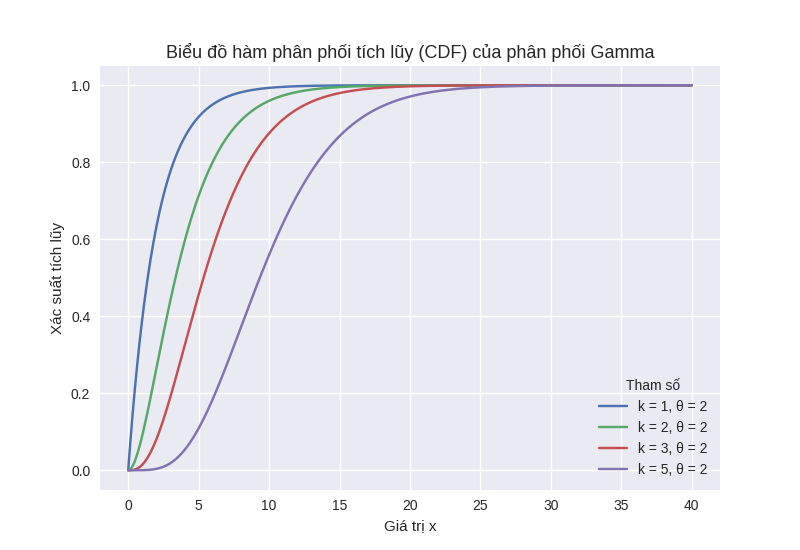
\includegraphics[width=0.7\tetextwidth]{images/Gamma Distribution-CDF.png} % Placeholder cho hình ảnh
		\caption{Hàm mật độ xác suất của Phân phối Gamma với các tham số khác nhau.}
		\label{fig:Gamma Distribution-CDF}
	\end{figure}
	
	\subsection{Ví dụ dữ liệu và bài toán thực tế}
		Thời gian spng} % Placeholder cho hình ảnh
		\caption{Hàm mật độ xác suất của Phân phối Gamma Nghịch đảo với các tham số khác nhau.}
		\label{fig:Inverse Gamma Distribution-PDF}
	\end{figure}
	
	Dưới đây là biểu đồ minh họa hàm xác suất tích lũy của phân phối Gamma Nghịch đảo
	
		\begin{figure}[h!]
		\centering
		\includegraphics[width=0.7\textwidth]{images/Inverse Gamma Distribution-CDF.png} % Placeholder cho hình ảnh
		\caption{Hàm mật độ xác suất của Phân phối Gamma Nghịch đảo với các tham số khác nhau.}
		\label{fig:Inverse Gamma Distribution-CDF}
	\end{figure}
	
	\subsection{Ví dụ dữ liệu và bài toán thực tế}
		Phân phối tiên nghiệm cho phương sai
		Trong thống kê Bayes, khi chúng ta cần đặt một phân phối tiên nghiệm cho tham số phương sai $\sigma^2$ của một phân phối chuẩn (normal distribution) hoặc các mô hình tuyến tính, phân phối Gamma Nghịch đảo là một lựa chọn phổ biến. Ví dụ, trong mô hình hồi quy tuyến tính, nếu chúng ta không có nhiều thông tin về phương sai của sai số, chúng ta có thể đặt một tiên nghiệm Gamma Nghịch đảo như $\text{InvGamma}(0.001, 0.001)$ để biểu thị sự không chắc chắn cao.
	
\section{Phân phối Beta (Beta Distribution)}
	Phân phối Beta là một phân phối xác suất liên tục được định nghĩa trên khoảng $[0, 1]$. Nó rất hữu ích để mô hình hóa các đại lượng có giá trị giới hạn trong khoảng này, chẳng hạn như xác suất, tỷ lệ hoặc tỷ lệ phần trăm.
	
	
	\subsection{Định nghĩa}
		Một biến ngẫu nhiên $X$ tuân theo phân phối Beta với hai tham số hình dạng $\alpha > 0$ và $\beta > 0$, ký hiệu $X \sim \text{Beta}(\alpha, \beta)$, có hàm mật độ xác suất được cho bởi:
		\[ f(x; \alpha, \beta) = \frac{x^{\alpha-1}(1-x)^{\beta-1}}{B(\alpha, \beta)} \quad \text{với } 0 \le x \le 1 \]
		Trong đó, $B(\alpha, \beta)$ là hàm Beta, được định nghĩa là $B(\alpha, \beta) = \frac{\Gamma(\alpha)\Gamma(\beta)}{\Gamma(\alpha+\beta)}$.
	
	\subsection{Hàm xác suất tích lũy (Cumulative Distribution Function - CDF)}
	Hàm xác suất tích lũy của phân phối Beta được biểu diễn thông qua hàm Beta không đầy đủ quy chuẩn (regularized incomplete beta function):
	\[ F(x; \alpha, \beta) = I_x(\alpha, \beta) = \frac{B_x(\alpha, \beta)}{B(\alpha, \beta)} \]
	Trong đó, $B_x(\alpha, \beta) = \int_0^x t^{\alpha-1}(1-t)^{\beta-1} dt$ là hàm Beta không đầy đủ.
	
	\subsection{Các đặc trưng thống kê}
	\begin{itemize}[leftmargin=*]
		\item \textbf{Miền giá trị:} $x \in [0, 1]$.
		\item \textbf{Giá trị kỳ vọng (Mean):} $E[X] = \frac{\alpha}{\alpha+\beta}$.
		\item \textbf{Phương sai (Variance):} $\text{Var}[X] = \frac{\alpha\beta}{(\alpha+\beta)^2(\alpha+\beta+1)}$.
		\item \textbf{Mode:}
		\[ \text{Mode} = \begin{cases} \frac{\alpha-1}{\alpha+\beta-2} & \text{nếu } \alpha > 1, \beta > 1 \\ 0 & \text{nếu } \alpha=1, \beta > 1 \\ 1 & \text{nếu } \alpha > 1, \beta=1 \\ \text{tất cả các giá trị trong (0,1)} & \text{nếu } \alpha=1, \beta=1 \text{ (phân phối đều)} \end{cases} \]
		\item \textbf{Median:} Không có dạng đóng. Đối với $\alpha = \beta$, median bằng $0.5$.
		\item \textbf{Tính chất đối xứng/lệch:}
		\begin{itemize}
			\item Nếu $\alpha = \beta$, phân phối đối xứng.
			\item Nếu $\alpha > \beta$, phân phối lệch trái.
			\item Nếu $\alpha < \beta$, phân phối lệch phải.
		\end{itemize}
	\end{itemize}
	
	\subsection{Biểu đồ minh họa}
	Dưới đây là biểu đồ minh họa hàm mật độ xác suất của phân phối Beta với các cặp tham số $\alpha, \beta$ khác nhau.
	
	\begin{figure}[h!]
		\centering
		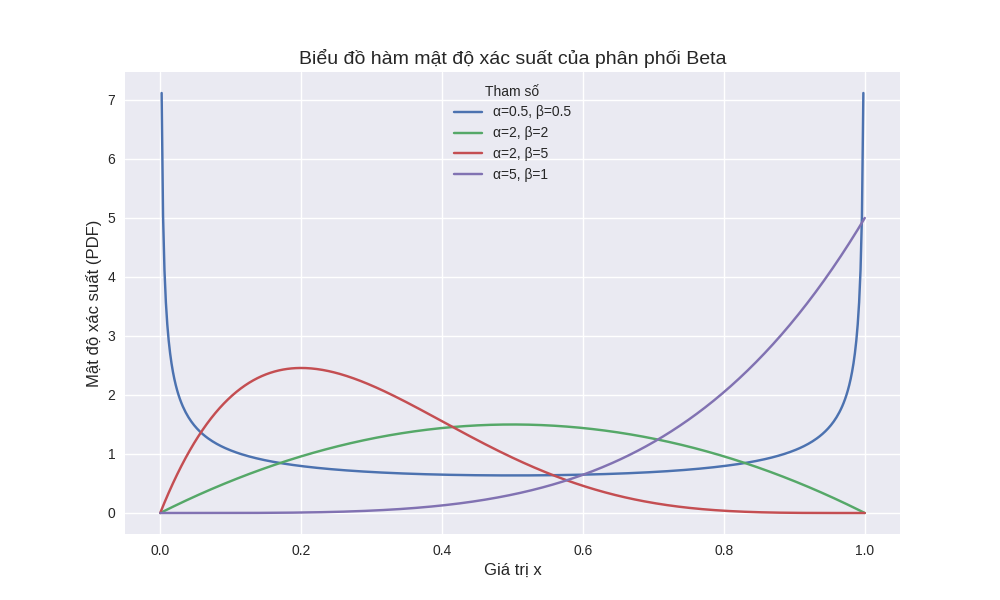
\includegraphics[width=0.7\textwidth]{images/Beta Distribution-PDF.png} % Placeholder cho hình ảnh
		\caption{Hàm mật độ xác suất của Phân phối Beta với các tham số khác nhau.}
		\label{fig:Beta Distribution-PDF}
	\end{figure}C
	
	Dưới đây là biểu đồ minh họa hàm xác suất tích lũy của phân phối Beta
	
		\begin{figure}[h!]
		\centering
		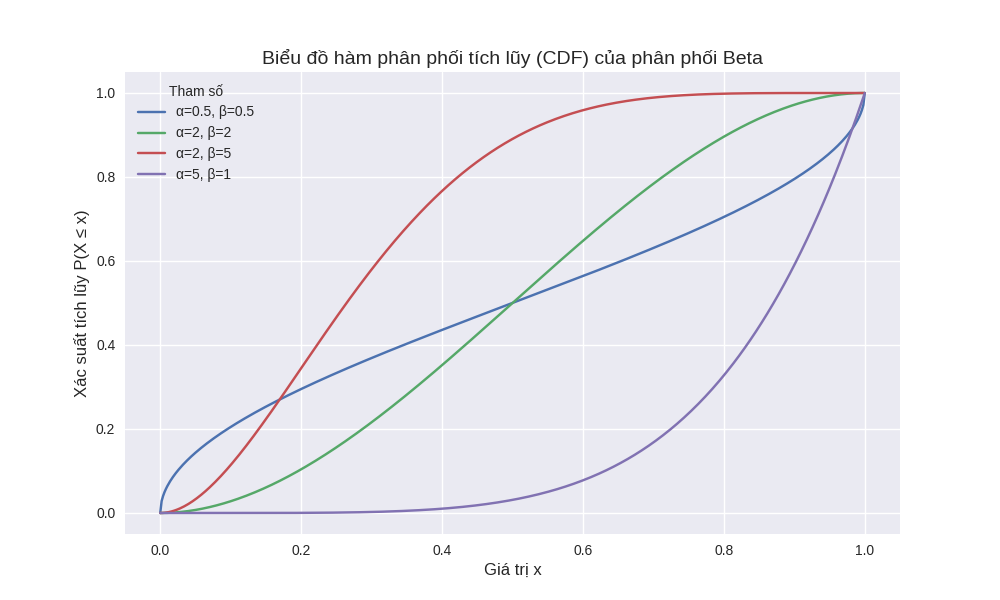
\includegraphics[width=0.7\textwidth]{images/Beta Distribution-CDF.pngpng} % Placeholder cho hình ảnh
		\caption{Hàm mật độ xác suất của Phân phối Beta với các tham số khác nhau.}
		\label{fig:Beta Distribution-CDF}
	\end{figure}
	
	\subsection{Ví dụ dữ liệu và bài toán thực tế}
		Phân phối tiên nghiệm cho xác suất Bernoulli
		Trong thống kê Bayes, phân phối Beta là liên hợp tiên nghiệm (conjugate prior) cho tham số $p$ của phân phối Bernoulli hoặc phân phối nhị thức (binomial distribution). Nếu chúng ta muốn ước lượng xác suất thành công $p$ của một thí nghiệm, chúng ta có thể đặt một tiên nghiệm Beta trên $p$. Ví dụ, $\text{Beta}(1,1)$ là tiên nghiệm không thông tin (uniform prior), trong khi $\text{Beta}(2,2)$ cho thấy chúng ta tin rằng $p$ có xu hướng ở gần $0.5$.
	
		Tỷ lệ phiếu bầu
		Giả sử chúng ta muốn mô hình hóa tỷ lệ phiếu bầu cho một ứng cử viên trong một cuộc bầu cử. Các giá trị tỷ lệ này nằm trong khoảng $[0, 1]$. Phân phối Beta có thể được sử dụng để biểu diễn sự không chắc chắn của chúng ta về tỷ lệ thực tế, dựa trên các cuộc thăm dò hoặc dữ liệu lịch sử.
	
\section{Phân phối Dirichlet (Dirichlet Distribution)}
	Phân phối Dirichlet là một phân phối xác suất đa biến liên tục trên một simplex tiêu chuẩn. Nó là tổng quát hóa của phân phối Beta cho nhiều hơn hai danh mục và thường được sử dụng làm phân phối tiên nghiệm cho các tham số của phân phối Categorical hoặc phân phối đa thức (multinomial distribution).
	
	\subsection{Định nghĩa}
		Một vector ngẫu nhiên $X = (X_1, X_2, \dots, X_K)$ tuân theo phân phối Dirichlet với tham số vector $\boldsymbol{\alpha} = (\alpha_1, \alpha_2, \dots, \alpha_K)$ với $\alpha_i > 0$ cho mọi $i$, ký hiệu $X \sim \text{Dirichlet}(\boldsymbol{\alpha})$, có hàm mật độ xác suất được cho bởi:
		\[ f(x_1, \dots, x_K; \alpha_1, \dots, \alpha_K) = \frac{1}{B(\boldsymbol{\alpha})} \prod_{i=1}^K x_i^{\alpha_i-1} \]
		với $x_i > 0$, $\sum_{i=1}^K x_i = 1$.
		
		Trong đó, $B(\boldsymbol{\alpha})$ là hàm Beta đa biến (multivariate beta function), được định nghĩa là:
		\[ B(\boldsymbol{\alpha}) = \frac{\prod_{i=1}^K \Gamma(\alpha_i)}{\Gamma\left(\sum_{i=1}^K \alpha_i\right)} \]
	
	\subsection{Hàm xác suất tích lũy (Cumulative Distribution Function - CDF)}
	Hàm xác suất tích lũy của phân phối Dirichlet không có dạng đóng đơn giản và phức tạp hơn nhiều so với các phân phối một biến. Thường không được sử dụng trực tiếp.
	
	\subsection{Các đặc trưng thống kê}
	\begin{itemize}[leftmargin=*]
		\item \textbf{Miền giá trị:} Simplex tiêu chuẩn $S_K = \left\{ (x_1, \dots, x_K) \mid x_i > 0, \sum_{i=1}^K x_i = 1 \right\}$.
		\item \textbf{Giá trị kỳ vọng (Mean):} Đối với từng thành phần $X_i$:
		\[ E[X_i] = \frac{\alpha_i}{\sum_{j=1}^K \alpha_j} \]
		\item \textbf{Phương sai (Variance):} Đối với từng thành phần $X_i$:
		\[ \text{Var}[X_i] = \frac{\alpha_i \left( \sum_{j=1}^K \alpha_j - \alpha_i \right)}{\left( \sum_{j=1}^K \alpha_j \right)^2 \left( \sum_{j=1}^K \alpha_j + 1 \right)} \]
		\item \textbf{Mode:} Đối với từng thành phần $X_i$:
		\[ \text{Mode}_i = \frac{\alpha_i-1}{\sum_{j=1}^K \alpha_j - K} \quad \text{(nếu tất cả } \alpha_i > 1 \text{)} \]
		\item \textbf{Median:} Không có dạng đóng.
		\item \textbf{Tính chất:} Phân phối Dirichlet là liên hợp tiên nghiệm cho phân phối Categorical và phân phối Đa thức.
	\end{itemize}
	
	\subsection{Biểu đồ minh họa}
	Việc minh họa hàm mật độ xác suất của phân phối Dirichlet yêu cầu các biểu đồ trên simplex. Đối với $K=3$, chúng ta có thể sử dụng biểu đồ tam giác.
	
	\begin{figure}[h!]
		\centering
		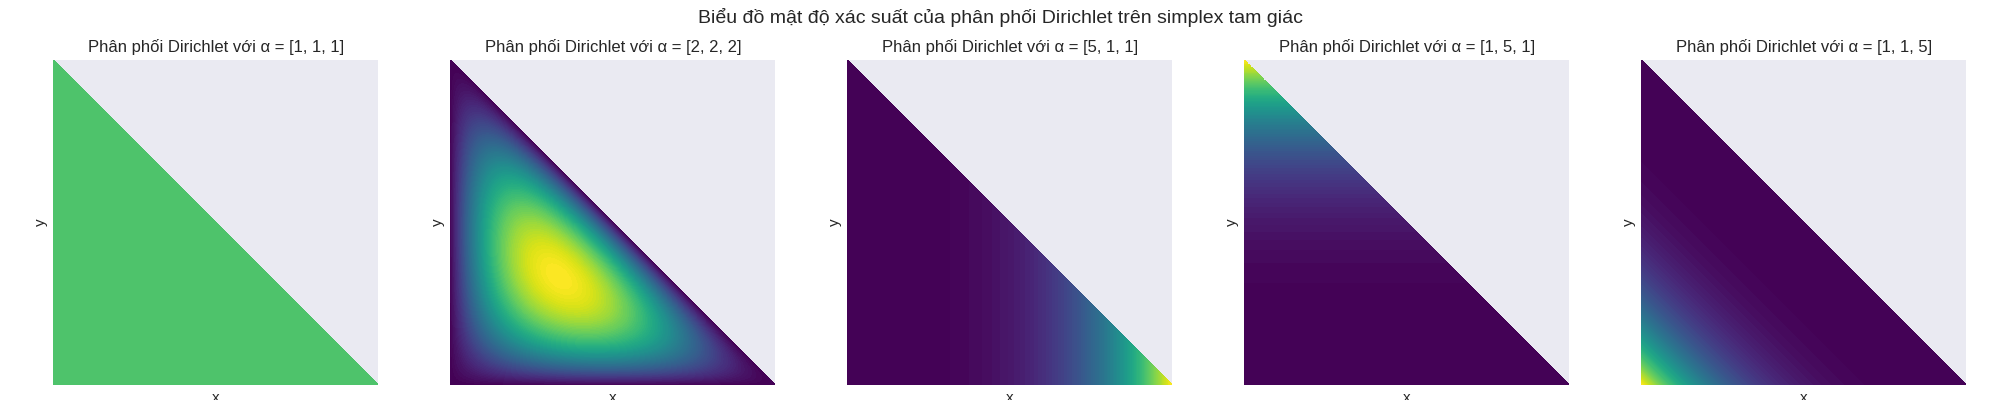
\includegraphics[width=0.7\textwidth]{images/Dirichlet Distribution-PDF.png} % Placeholder cho hình ảnh
		\caption{Hàm mật độ xác suất của Phân phối Dirichlet với $K=3$ và các tham số khác nhau.}
		\label{fig:pngDirichlet Distribution-PDF}
	\end{figurell}
	
	Biểu đồ minh hoạt hàm xuất sắc tích lũy của phân phối Dirichlet
	
	\begin{figure}[h!]
		\centering
		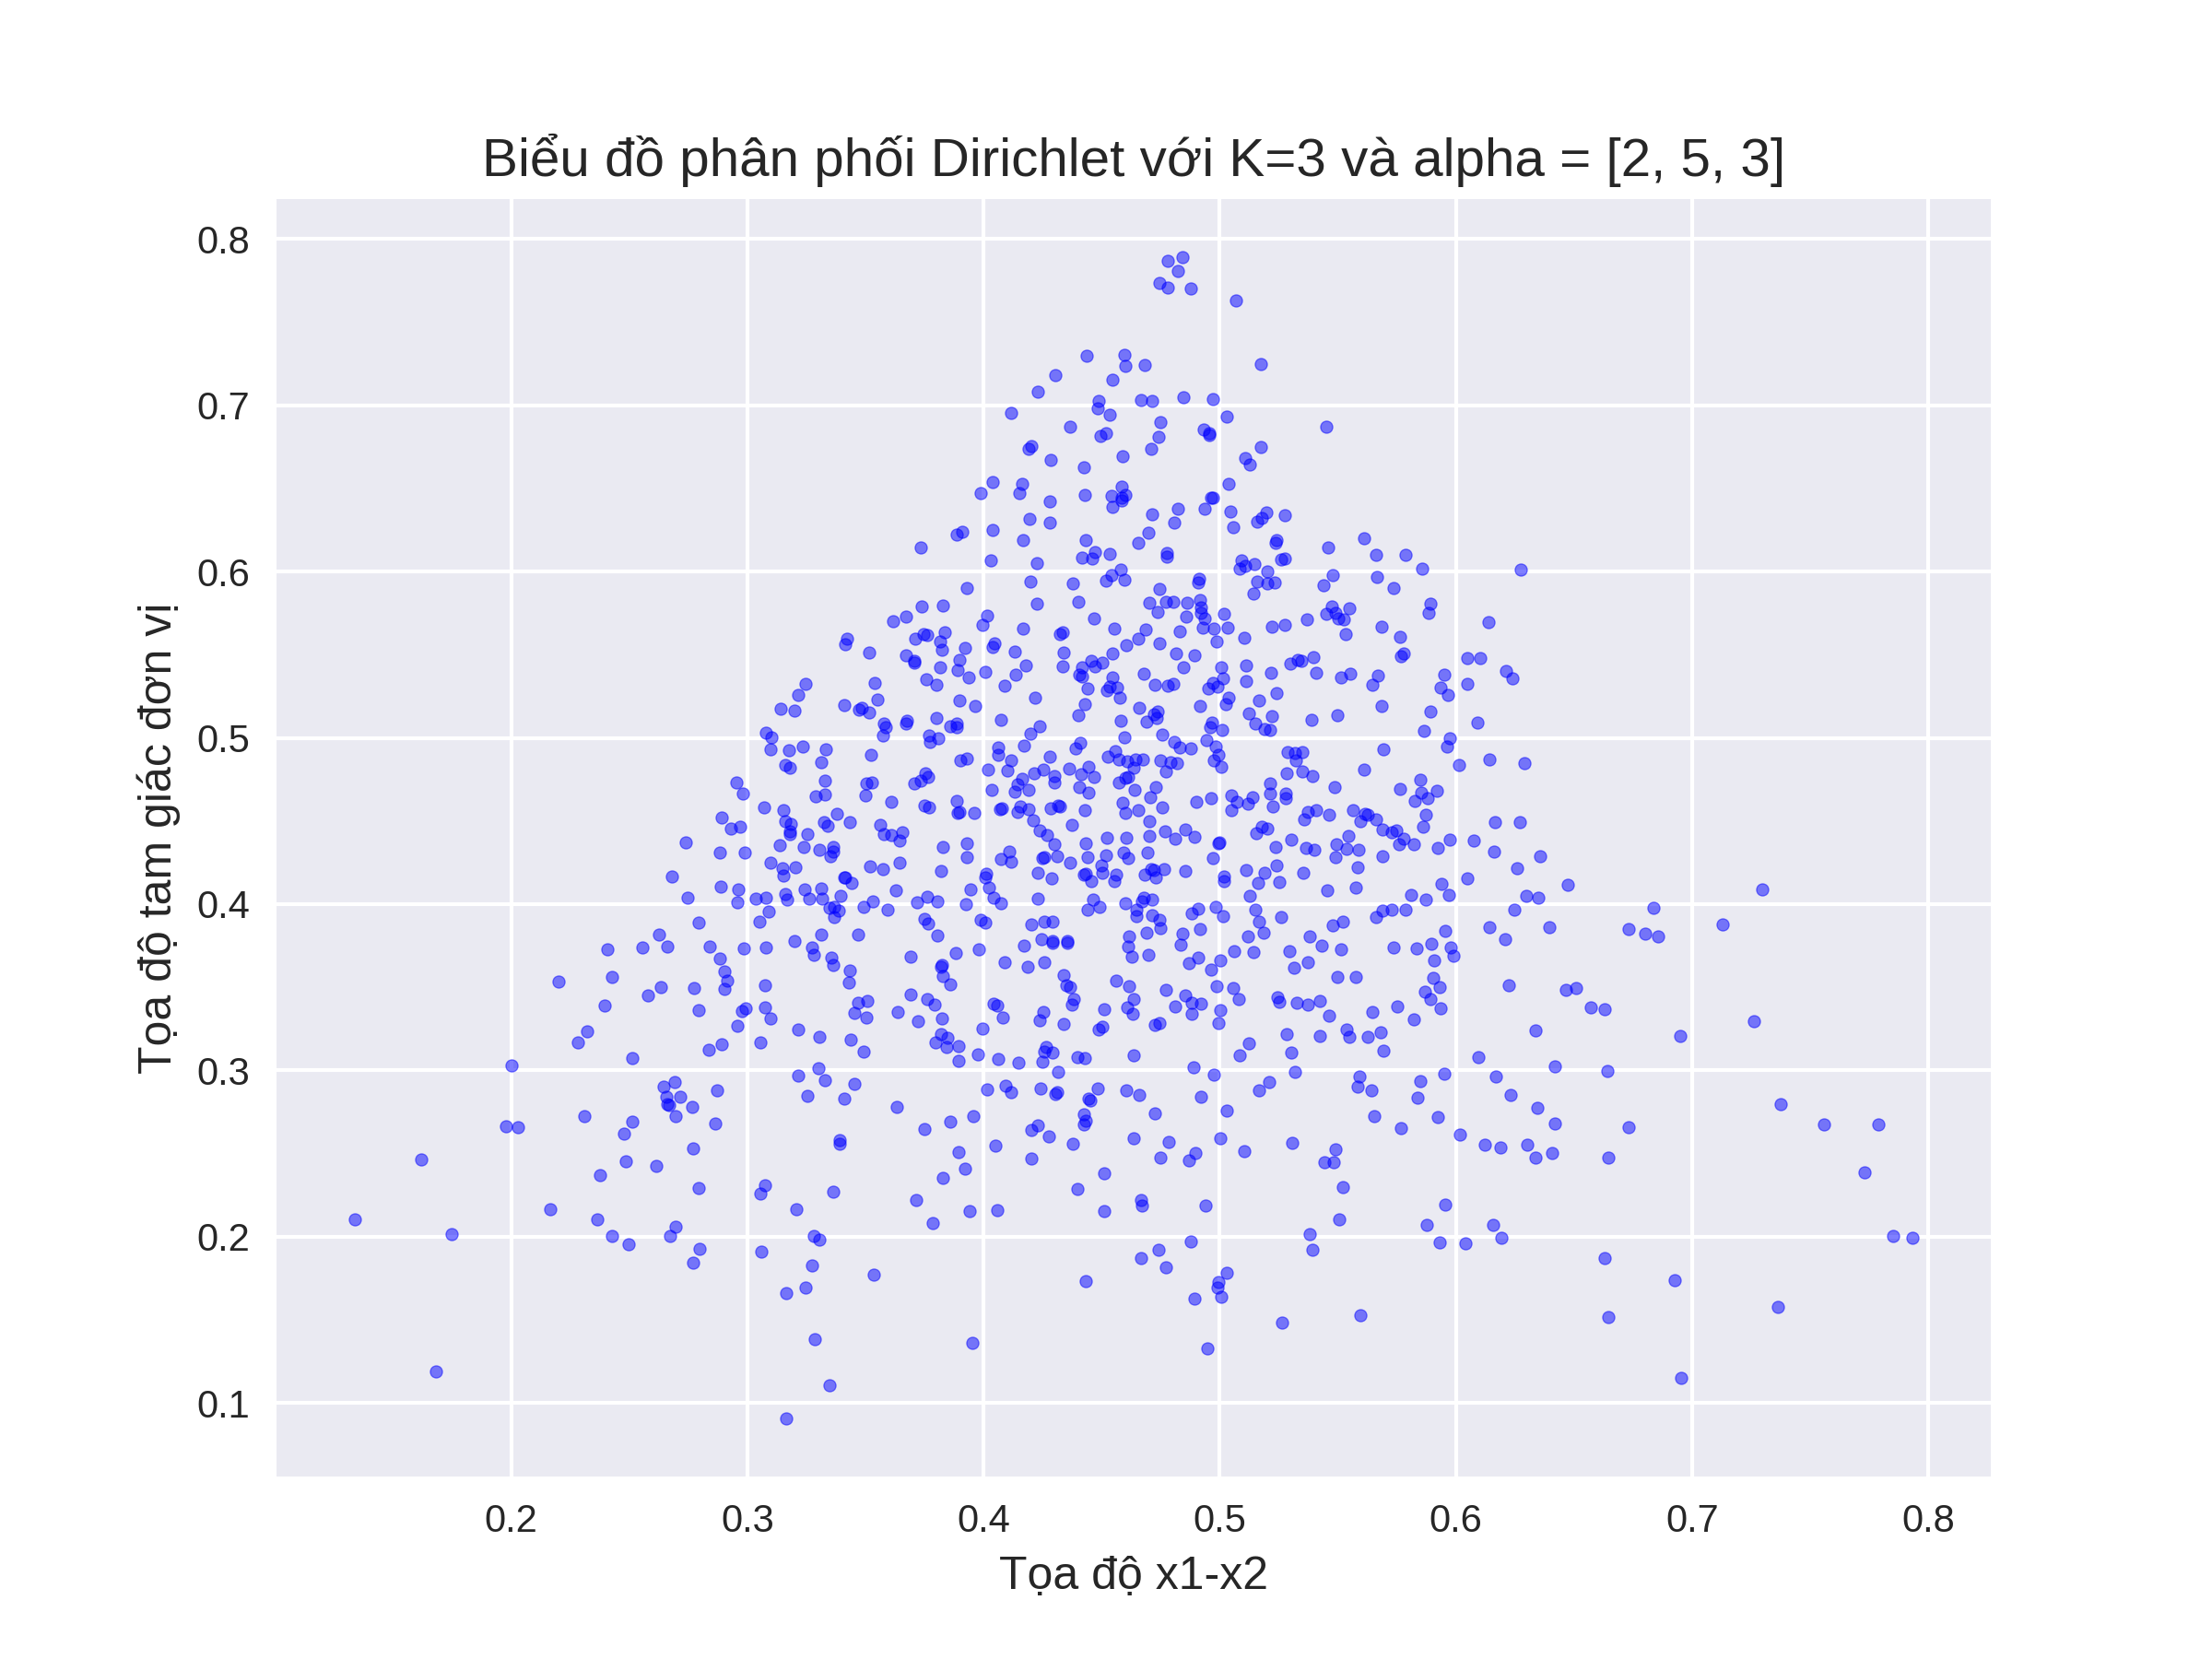
\includegraphics[width=B0.7\textwidth]{images/Dirichlet Distribution-CDF.png} % Placeholder cho hình ảnh
		\caption{Hàm mật độ xác suất của Phân phối Dirichlet với $K=3$ và các tham số khác nhau.}
		\label{fig:pngDirichlet Distribution-CDF}
	\end{figurell}
	
	\subsection{Ví dụ dữ liệu và bài toán thực tế}
		Phân phối tiên nghiệm cho phân loại văn bản
		Trong mô hình hóa chủ đề (topic modeling) như Latent Dirichlet Allocation (LDA), phân phối Dirichlet được sử dụng làm phân phối tiên nghiệm cho hai cấp độ:
		\begin{itemize}
			\item Phân phối các chủ đề trên một tài liệu (document-topic distribution).
			\item Phân phối các từ trên một chủ đề (topic-word distribution).
		\end{itemize}
		Ví dụ, $\text{Dirichlet}(\boldsymbol{\alpha})$ với $\alpha_i$ nhỏ (ví dụ, $\alpha_i=0.1$) sẽ khuyến khích các phân phối thưa, nghĩa là mỗi tài liệu có xu hướng chỉ nói về một vài chủ đề chính.
	
		Phân phối tiên nghiệm cho xác suất đa thức
		Giả sử chúng ta có một thí nghiệm với $K$ kết quả có thể xảy ra, mỗi kết quả có xác suất $p_i$. Vector $(p_1, \dots, p_K)$ với $\sum p_i = 1$ có thể được mô hình hóa bằng phân phối Dirichlet. Ví dụ, tỷ lệ các loại sản phẩm khác nhau được bán trong một siêu thị.
